\documentclass[12pt]{standalone}
\usepackage{tikz}
\usetikzlibrary{calc, arrows.meta, decorations.pathreplacing}

\begin{document}

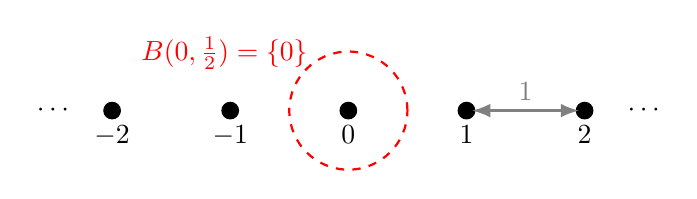
\begin{tikzpicture}[baseline={(0,0)}, scale=1.5]


% Define the coordinates of the points
\coordinate (y2) at (-2,0);
\coordinate (y1) at (-1,0);
\coordinate (x0) at (0,0);
\coordinate (x1) at (1,0);
\coordinate (x2) at (2,0);
\coordinate (e) at (2.5, 0);
\coordinate (f) at (-2.5, 0);

% Define radii for the open balls around x and y (both equal to d(x, y) / 2)
\def\radius{0.5}  % Set r1 = r2 = d(x, y) / 2

% Draw the open balls as circles with dashed boundaries
\draw[red, thick, dashed] (x0) circle (\radius) node[above left=11pt] {$B(0, \frac{1}{2}) = \{0\}$};
% \draw[red, thick, dashed] (y) circle (\radius) node[above right=4pt] {$B(y, \frac{d(x,y)}{2})$};

% Draw the points x and y
\filldraw[black] (y2) circle (2pt) node[below, yshift=-2pt] {$-2$};
\filldraw[black] (y1) circle (2pt) node[below, yshift=-2pt] {$-1$};
\filldraw[black] (x0) circle (2pt) node[below, yshift=-2pt] {$0$};
\filldraw[black] (x1) circle (2pt) node[below, yshift=-2pt] {$1$};
\filldraw[black] (x2) circle (2pt) node[below, yshift=-2pt] {$2$};
\node at (e) {$\cdots$};
\node at (f) {$\cdots$};

% Draw the line connecting x and y
\draw[thick, gray, {Latex}-{Latex}, shorten <= 2pt, shorten >= 2pt ] (x1) -- (x2) node[midway, above] {$1$};

\end{tikzpicture}
\end{document}
